\documentclass[11pt]{article}
\usepackage[T1]{fontenc}
\usepackage{lmodern,amsmath,amssymb,amsthm,mathtools,booktabs,microtype,graphicx}
\usepackage[letterpaper,left=1.05in,right=1.05in,top=0.88in,bottom=0.9in]{geometry}
\usepackage{xcolor}
\definecolor{ink}{HTML}{193B56}
\usepackage[colorlinks=true,linkcolor=ink,urlcolor=ink,citecolor=ink,pdfauthor={OpenAI},pdftitle={Sharp-window transport of Dirichlet zeros}]{hyperref}
\usepackage{fancyhdr}
\pagestyle{fancy}\fancyhf{}\fancyhead[L]{\small\itshape Sharp-window transport of Dirichlet zeros}\fancyhead[R]{\small Research note}\fancyfoot[C]{\thepage}
\setlength{\headheight}{14pt}
\newtheorem{theorem}{Theorem}
\newtheorem{lemma}[theorem]{Lemma}
\newtheorem{corollary}[theorem]{Corollary}
\DeclareMathOperator{\Log}{Log}\DeclareMathOperator{\tr}{tr}\DeclareMathOperator{\diag}{diag}
\newcommand{\R}{\mathbb R}\newcommand{\C}{\mathbb C}
\newcommand{\dd}{\,\mathrm d}\newcommand{\ii}{\mathrm i}
\newcommand{\Imn}{\operatorname{Im}}\newcommand{\Ren}{\operatorname{Re}}
\newcommand{\id}{\mathbf1}\newcommand{\norm}[1]{\left\lVert#1\right\rVert}
\newcommand{\abs}[1]{\left\lvert#1\right\rvert}
\newcommand{\ph}{\Phi}\newcommand{\Gm}{G_0}
\newcommand{\repo}[1]{\href{https://github.com/VladimirReshetnikov/ProveIt/blob/f6b5955e13bcefb2760480e7b823eba55ed2383e/Analysis/GeneralizedRiemannHypothesis/#1}{\nolinkurl{#1}}}
\setlength{\emergencystretch}{2em}
\allowdisplaybreaks[1]
\begin{document}
\thispagestyle{plain}
\begin{center}
{\small\sffamily\color{ink} ANALYTIC NUMBER THEORY}\par\vspace{7pt}
{\LARGE\bfseries Sharp-window transport of Dirichlet zeros}\par\vspace{5pt}
{\large A local Cauchy law and a convergent displacement remainder}\par\vspace{9pt}
{\small November 27, 2026}
\end{center}

\begin{abstract}
We prove a sharp-interval formula for the spectral shift of Hermitian couplings of completed Dirichlet functions, using Dirichlet GRH. The formula has a dimension-free endpoint error, uniform in the conductors and both coupling matrices. For a single character it gives a relative Cauchy law simultaneously for every Borel set of values of the real logarithmic derivative, on every interval of length $H$ with $H\log\log(qT)\to\infty$. The error scales with the probability of the set, even arbitrarily far in the tails. For a fixed coupling, subtracting an explicit function of the conductors and matrices from the accumulated displacement leaves a finite limit, with error $O(1/(\log T\log\log T))$. An elementary rectangle estimate for the Cayley transform and a positive combination of Poisson kernels give the endpoint control.
\end{abstract}

\section{A scalar statement}
Put $F(t)=\xi(1/2+\ii t)$ for the Riemann zeta function. For a primitive nonprincipal Dirichlet character $\chi$ of conductor $q$ and parity $a\in\{0,1\}$, put
\[
 \Lambda_\chi(s)=(q/\pi)^{(s+a)/2}\Gamma((s+a)/2)L(s,\chi),
 \qquad F(t)=\eta_\chi^{-1}\Lambda_\chi(1/2+\ii t),
\]
where $\eta_\chi^2$ is the root number and $|\eta_\chi|=1$. Here $\xi(s)=\tfrac12s(s-1)\pi^{-s/2}\Gamma(s/2)\zeta(s)$ and we assign $q=1$ to this input. The functional equation makes $F$ real on $\R$, including for complex characters. Write $g=F'/F$ with the derivative taken in the ordinate $t$. For $t>2\pi/q$ define
\[
 d_q(t)=\tfrac12\log(qt/(2\pi)),\qquad
 p_{q,t}(v)=\frac{1}{\pi}\frac{d_q(t)}{(v+\pi/4)^2+d_q(t)^2},\qquad
 p^*_{q,T}(v)=\frac{1}{\pi}\frac{d_q(T)}{v^2+d_q(T)^2}.
\]
Both densities integrate to one. For a density $p$ write $p(E)=\int_E p(v)\dd v$.

\begin{theorem}[Uniform local Cauchy law]\label{th:scalar}
Use RH for the zeta input and Dirichlet GRH for the character inputs. For all sufficiently large $T$, put $d=d_q(T)$. For every interval $I\subset[T,2T]$ of length $H$ and every Borel set $E\subset\R$,
\begin{equation}\label{eq:scalar}
 \left|\, |\{t\in I:g(t)\in E\}|-\int_I p_{q,t}(E)\dd t\,\right|
 \le \frac{C}{\log d}\,p^*_{q,T}(E).
\end{equation}
The constant and the threshold for $T$ are absolute. In particular if $H>0$ and $p^*_{q,T}(E)>0$ the probability for uniform $t\in I$ equals
\begin{equation}\label{eq:rel}
 p^*_{q,T}(E)\left(1+O\left(d^{-1}+(H\log d)^{-1}\right)\right).
\end{equation}
\end{theorem}

For example, take $q=1$, $I=[T,T+H]$, $H=(\log\log T)^{-1/2}$, and $E=[e^T,e^T+e^{-T}]$. The length of the set of ordinates with $g(t)\in E$ is asymptotic to $H d_1(T)e^{-3T}/\pi$. Both the time interval and the proportion of qualifying times tend to zero. Lebesgue length is essential here.

\paragraph{Relation to the source.}
The repository snapshot \cite{repo} merges 184 reports into an 851-page article. Its section on transport proves a determinant-phase identity, the first-order growth on intervals proportional to $T$, and an all-orders expansion after Poisson smoothing. Its scalar local Cauchy theorem permits arbitrarily narrow value intervals whose rescaled endpoints approach a finite value, with a time interval proportional to $T$. Its discussion explicitly leaves the coefficient expansion on sharp time intervals unstated. We use the same spectral shift. Our contributions are the endpoint estimate, the uniform local law \eqref{eq:scalar}, and the convergent renormalization of Theorem~\ref{th:global}. Section~\ref{sec:prior} identifies the exact dependencies and literature. All results below are analytic proofs; the Lean input is the upstream real-zero theorem \cite{lean}.

\section{The matrix statement}
Let $F_1,\ldots,F_n$ be any finite list of the above functions, with repetitions allowed. Put $g_j=F_j'/F_j$, $G(z)=\diag(g_j(z))$, and let $A=A^*$, $B=B^*\succeq0$ be complex Hermitian matrices. For real $x$ outside the discrete set of input and output zeros define
\[
 \sigma(x)=n_+(A+B+G(x))-n_+(A+G(x)).
\]
Here $n_+$ counts positive eigenvalues with multiplicity. The output attached to $A$ is the entire function
\[
 \mathcal P_A(z)=\det\bigl(\diag(F_j(z))A+\diag(F'_j(z))\bigr).
\]
For a rank-one update, $\sigma$ is the indicator of intervals running from an old output zero to a new one after common zeros are canceled. Thus $\int_I\sigma$ measures displacement clipped to $I$. A general positive update is a sum of rank-one updates and the inertia differences telescope. Added graph edges correspond to $B=w(e_j-e_k)(e_j-e_k)^*$.

For a diagonal $Z$ with $\Imn Z\prec0$ define the complex phase
\begin{equation}\label{eq:phase}
 \ph(Z)=\int_0^1\tr\bigl(B(A+uB+Z)^{-1}\bigr)\dd u.
\end{equation}
It is a logarithm of $\det(A+B+Z)/\det(A+Z)$ by differentiation in $u$. This definition fixes the branch for all ranks. Let
\begin{align}
 D(t)&=\diag(d_{q_j}(t)), &D&=D(T), &d&=\min_j D_{jj},\notag\\
 W&=\Imn\ph(-\ii D),&
 \rho(t)&=\pi^{-1}\Imn\ph(-\tfrac\pi4\id-\ii D(t)).\label{eq:rho}
\end{align}
Throughout $\id$ denotes the identity matrix. In particular $W>0$ if $B\ne0$.

\begin{theorem}[Sharp interval estimate]\label{th:matrix}
Under Dirichlet GRH, for all $T\ge T_0$ and all intervals $I\subset[T,2T]$,
\begin{equation}\label{eq:matrix}
 \left|\int_I\sigma(t)\dd t-\int_I\rho(t)\dd t\right|
 \le C\,\frac{W}{\log d},\qquad
 \pi\rho(t)=W\bigl(1+O(d^{-1})\bigr)\quad(T\le t\le2T).
\end{equation}
The constants $T_0,C$ and the implied constant are absolute, independent of $n$, the characters, the conductors, $A$, and $B$. These data may all vary with $T$.
\end{theorem}

For fixed data, $W\sim 2\tr(B)/\log T$ if $B\ne0$. The absolute error in \eqref{eq:matrix} is then $O(1/(\log T\log\log T))$ for every endpoint pair in a dyadic interval. Uniformity in $A$ and $B$ is what gives the much finer error for a rare scalar event.

\section{Three estimates for the proof}
\subsection{The positive boundary phase}
A real entire function of order at most one with only real zeros has a real genus-at-most-one Hadamard product. For $z=x+\ii y$, $y>0$, it gives
\[
 -\Imn g_j(z)= y\sum_{F_j(\gamma)=0}\frac{m_\gamma}{|z-\gamma|^2}>0,
\]
where the sum is over distinct zeros and $m_\gamma$ is the multiplicity. The completed functions have zeros and Dirichlet GRH places them all on the real ordinate axis. Thus $A+G(z)$ is invertible. Write $B=VV^*$ with $V$ of full column rank $r$. The matrix $H_0=V^*(A+G(z))^{-1}V$ has positive definite imaginary part. The determinant lemma, or integration along $u$, gives $\ph(G(z))=\tr\log(\id+H_0)$ with the principal matrix logarithm. Its imaginary part lies between $0$ and $r\pi$ if $r>0$. At a regular real point the boundary value of $\Imn\ph(G)/\pi$ is $n_-(\id+H_0)$. Taking Schur complements in the Hermitian matrix with diagonal blocks $A+G(x),-\id$ and off-diagonal blocks $V,V^*$ yields $n_-(\id+H_0)=\sigma(x)$. The bounded harmonic Poisson formula consequently gives
\begin{equation}\label{eq:poisson}
 (P_y*\sigma)(x)=\pi^{-1}\Imn\ph(G(x+\ii y)),\qquad
 P_y(s)=\frac{y}{\pi(s^2+y^2)}.
\end{equation}
This is the repository's displacement identity \cite{repo}. The case $B=0$ is immediate in all formulas.

\subsection{Comparing resolvents without losing the size of the event}
Put $A'=D^{-1/2}AD^{-1/2}$, $B'=D^{-1/2}BD^{-1/2}$ and $Z'=D^{-1/2}ZD^{-1/2}$. Equation~\eqref{eq:phase} is unchanged by applying this congruence to all its arguments. With $X=A'+uB'$ we obtain
\begin{equation}\label{eq:W}
 W=\int_0^1\tr\bigl(B'(\id+X^2)^{-1}\bigr)\dd u.
\end{equation}
Equivalently $W=\tr(\arctan(A'+B')-\arctan A')$, by the path derivative of the trace, or by the determinant phase at $-\ii\id$.

\begin{lemma}\label{lem:res}
If $\norm{Z'_j+\ii\id}\le1/2$ for $j=1,2$, then
\[
 |\ph(Z_1)-\ph(Z_2)|\le4 W\norm{Z'_1-Z'_2}.
\]
In particular $\Imn\ph(Z_1)\ll W$ under this norm condition.
\end{lemma}
\begin{proof}
Let $R_*=(X-\ii\id)^{-1}$, $R_j=(X+Z'_j)^{-1}$. Factoring the inverse with $\norm{R_*}\le1$ gives
$\norm{R_j B'^{1/2}}_{\mathrm{HS}}\le2\norm{R_*B'^{1/2}}_{\mathrm{HS}}$.
The adjoints satisfy the same bound since $R_*$ is normal and $R_*^*R_*=(\id+X^2)^{-1}$. In
$R_1-R_2=R_1(Z'_2-Z'_1)R_2$, apply Hilbert--Schmidt Cauchy--Schwarz after placing $B'^{1/2}$ on the two outside factors. The square of the reference norm integrates to $W$. For the last assertion take $Z_2=-\ii D$.
\end{proof}

\subsection{A rectangle estimate near the real axis}
Use the principal logarithm and set
\[
 \Gm(z)=-\ii\diag\left(\tfrac12\log(q_j/(2\pi))+\tfrac12\Log(-\ii z)\right).
\]
For $t>0$ its boundary value equals $-\pi\id/4-\ii D(t)$. The real shift $-\pi/4$ comes from the argument of $-\ii t$. Define $Y=2+4\log(2T)$.

\begin{lemma}\label{lem:strip}
There are absolute $c,C_0>0$ such that for $T\ge T_0$, $T\le t\le2T$, $h=C_0/\log d$ and $z=t+\ii y$,
\begin{align}
 \norm{D^{-1/2}(G-\Gm)(z)D^{-1/2}}
 &\ll e^{-c y\log d}+d^{-1} && (h\le y\le1),\label{eq:low}\\
 &\ll (T^{-1}+2^{-y})/d && (1\le y\le Y).\label{eq:high}
\end{align}
Each normalized matrix $G(z),\Gm(z)$ differs from $-\ii\id$ by at most $1/2$ in norm throughout $h\le y\le Y$. The same assertion holds for $\Gm$ down to $y=0$.
\end{lemma}
\begin{proof}
Set $s=1/2-\ii z$. The functional equation gives $g_j(z)=-\ii\Lambda_{\bar\chi_j}'(s)/\Lambda_{\bar\chi_j}(s)$, with $\xi$ in the zeta case. For $y\ge1$, the absolutely convergent logarithmic derivative of the Euler product is $O(2^{-y})$ uniformly in the character, since $\sum_{m\ge2}\Lambda(m)m^{-3/2}<\infty$. The gamma contribution is $\tfrac12\log(q_j/\pi)+\tfrac12\psi((s+a_j)/2)$. Stirling's formula $\psi(w)=\Log w+O(1/|w|)$ gives $g_j(z)=(\Gm)_{jj}(z)+O(|z|^{-1}+2^{-y})$. The rational terms $1/s+1/(s-1)$ for $\xi$ obey the same bound. This proves \eqref{eq:high}. On this rectangle $\Gm(z)+\ii D=O(1)$ in operator norm, uniformly since $Y=O(\log T)$.

Write $d_j=D_{jj}$. The Cayley transform $w_j=(g_j+\ii d_j)/(g_j-\ii d_j)$ is holomorphic and has modulus at most one above the real axis. At height $1$ and $|x-t|\le1$, the estimates just proved yield $|w_j(x+\ii)|\le K/d_j$ for an absolute $K$. On the rectangle $|x-t|\le1$, $0\le y\le1$, the harmonic function
\[
 v(x,y)=\frac{\cos(\pi(x-t)/2)\sinh(\pi y/2)}{\sinh(\pi/2)}
\]
vanishes on its sides and bottom and takes values in $[0,1]$ on its top. The subharmonic maximum principle applied to $\log|w_j|+v\log(d_j/K)$ shows
$|w_j(t+\ii y)|\le\exp(-c y\log d_j)$. Real poles of $g_j$ are removable in $w_j$. Choosing $C_0$ sufficiently large, inversion of the Cayley transform gives
$|g_j/d_j+\ii|\le 2|w_j|/(1-|w_j|)\le1/2$ for $h\le y\le1$, as well as \eqref{eq:low}. Increase $T_0$ so that $2h<1$ and the remaining norm assertions follow.
\end{proof}

\section{Removing the smoothing}
Define
\[
 K_h(s)=2P_h(s)-P_{2h}(s)=\frac{6h^3}{\pi(s^2+h^2)(s^2+4h^2)}.
\]
It is nonnegative and has integral one. For $r\ge0$ its one-sided tail satisfies
\[
 \int_r^\infty K_h(s)\dd s\ll\min(1,(h/r)^3)\ll hP_h(r),
\]
with the continuous interpretation at $r=0$. For $I=[a,b]$, a change between $\id_I(s)$ and $\id_I(s-u)$ requires crossing $a$ or $b$. Integration first in $u$ therefore gives
\begin{equation}\label{eq:clip}
 \left|\int_I(f-K_h*f)\right|
 \ll h\big((P_h*f)(a)+(P_h*f)(b)\big)
\end{equation}
for every bounded nonnegative $f$. Values at the endpoints have zero Lebesgue measure. The extra decay of $K_h$ is essential in this comparison with $P_h$.

\begin{proof}[Proof of Theorem~\ref{th:matrix}]
Use $h$ from Lemma~\ref{lem:strip}. Equations~\eqref{eq:poisson}, \eqref{eq:clip} and Lemma~\ref{lem:res} show that replacing $\sigma$ by $K_h*\sigma$ costs $O(hW)$. Its integral equals $1/\pi$ times the imaginary part of the horizontal integrals of $\ph(G)$ at heights $h,2h$, with coefficients $2,-1$.

Write $J(z)=\ph(G(z))-\ph(\Gm(z))$. For $\eta=h,2h$, integrate $J$ around $[a,b]+\ii[\eta,Y]$. It is holomorphic there since the imaginary parts are negative definite. At either vertical side, Lemmas~\ref{lem:res} and~\ref{lem:strip} bound its integral in absolute value by
\[
 CW\left(\int_h^1(e^{-cy\log d}+d^{-1})\dd y+
    d^{-1}\int_1^Y(T^{-1}+2^{-y})\dd y\right)\ll W/\log d.
\]
The top side costs $O(W/d)$ since $b-a\le T$ and $T2^{-Y}\le1$. Cauchy's theorem gives the same $O(W/\log d)$ bound on the integral of $J$ along the bottom. This step bounds an integral of the arithmetic remainder over a long interval by its values near the endpoints.

Finally, $\norm{D^{-1/2}(\Gm(t+\ii\eta)-\Gm(t))D^{-1/2}}\ll\eta/(Td)$, by differentiation of the logarithm. Lemma~\ref{lem:res} bounds the integrated change by $O(W\eta/d)$. The coefficients $2,-1$ sum to one, leaving $\int_I\rho$. The pointwise formula in \eqref{eq:matrix} follows from the same lemma since $\norm{D^{-1/2}(\Gm(t)+\ii D)D^{-1/2}}\ll1/d$.
\end{proof}

\begin{proof}[Proof of Theorem~\ref{th:scalar}]
For an interval of values $(u,v)$, take $n=1$, $A=-v$ and $B=v-u$. Outside a discrete set $\sigma=\id_{\{u<g<v\}}$. Direct integration of \eqref{eq:phase} gives
$W=\pi p^*_{q,T}((u,v))$ and $\rho(t)=p_{q,t}((u,v))$. Apply Theorem~\ref{th:matrix}. Both the occupation measure and the model measure are finite. Interval endpoints have zero mass for each, since $g$ is a nonconstant meromorphic function. By additivity the upper and lower measure inequalities in \eqref{eq:scalar} extend to finite disjoint unions of intervals, then to all Borel sets by the monotone class theorem. Finally the pointwise matrix estimate gives the relative version on intervals of values, and the same argument extends it to all Borel sets.
\end{proof}

\paragraph{A weighted count of level crossings.}
On each pole-free component of $I$, $g'(x)=-\sum_\gamma m_\gamma/(x-\gamma)^2<0$. Change of variables gives the density of the occupation measure at almost every $v$ as
\[
 w_I(v)=\sum_{x\in I^{\circ}:g(x)=v}\frac1{|g'(x)|}.
\]
Theorem~\ref{th:scalar} is equivalently the pointwise estimate
$|w_I(v)-\int_I p_{q,t}(v)\dd t|\le C p^*_{q,T}(v)/\log d$ almost everywhere. For $v=0$, the solutions are critical points of $F$ off its zeros; other levels give the corresponding zeros of $F'-vF$. The estimate extends by continuity at every level which is a regular value of the interval endpoints in the sense that it differs from their finite $g$-values.

\paragraph{Recovering the zero count from the far tail.}
Take $E=(v,\infty)$ and assume neither endpoint of $I$ is a pole. As $v\to+\infty$, $v|\{x\in I:g(x)>v\}|\to\sum_{\gamma\in I}m_\gamma$ since $g(x)=m_\gamma/(x-\gamma)+O(1)$ at each pole. Multiplying \eqref{eq:scalar} by $v$ yields
\[
 \left|\sum_{\gamma\in I}m_\gamma-\frac1\pi\int_I d_q(t)\dd t\right|\ll d/\log d.
\]
This recovers the order of the classical GRH discrepancy for the zero count. Sharper constants for that problem are known \cite{ccm}. The new estimate treats the entire value line in one measure inequality.

\clearpage
\section{A finite part for infinite zero transport}
\begin{theorem}[Convergent displacement remainder]\label{th:global}
Fix the functions and $A,B$, with $B\succeq0$. Fix $t_0$ sufficiently large for $D(t)$ to be positive definite above $t_0$. There is a real constant $C(t_0)$ such that
\begin{equation}\label{eq:global}
 \int_{t_0}^T \sigma(t)\dd t
   =\int_{t_0}^T \rho(t)\dd t+C(t_0)
      +O\left(\frac1{\log T\log\log T}\right).
\end{equation}
For $B\ne0$ the improper integral defining $C(t_0)$ is conditionally convergent.
\end{theorem}

A dyadic summation of Theorem~\ref{th:matrix} would give the divergent error series $\sum_{k\ge2}1/(k\log k)$. A separate contour argument makes the bound uniform all the way from $a$ to an arbitrary $b\ge a$.

\begin{proof}
All implied constants here may depend on the fixed data. Use one more term of Stirling's formula. Put $G_1(z)=\Gm(z)+C_1/z$, where $C_1$ is diagonal with real entries
\[
 c_j=a_j/2-1/4+2\id_{\{F_j=F_\zeta\}},\qquad a_\zeta=0 .
\]
The indicator here identifies the zeta input, independently of notation for the function. Indeed for $w=(1/2+a_j-\ii z)/2$, insert $\psi(w)=\Log w-1/(2w)+O(|w|^{-2})$ in the logarithmic derivative. The zeta polynomial contributes $-\ii(1/s+1/(s-1))=2/z+O(|z|^{-2})$ with $s=1/2-\ii z$. Thus, uniformly for $x=\Ren z$ large and $y=\Imn z\ge1$,
\begin{equation}\label{eq:stir2}
 \norm{G(z)-G_1(z)}\ll 2^{-y}+|z|^{-2}.
\end{equation}
Uniformity holds to arbitrarily large $y$, since $s+a_j$ remains in the closed right half-plane and $|z|\ge x$.

Take $a$ large and $h=C_2/\log\log a$ with $C_2$ a sufficiently large fixed constant. For every $t\ge a$, the proof of Lemma~\ref{lem:strip}, now frozen at $T=t$, applies for $h\le y\le1$ since $h\ge C_0/\log(\min_j d_{q_j}(t))$. In this range the resolvent calculation, with scale $\ell_t=\tfrac12\log t$ and fixed matrices, gives
\begin{equation}\label{eq:tailvertical}
 |\ph(G(t+\ii y))-\ph(G_1(t+\ii y))|
 \ll \frac{e^{-c y\log\log t}}{\log t}+\frac1{(\log t)^2}.
\end{equation}
Here $W_t\ll1/\log t$ and the additional diagonal perturbation $C_1/z$ is $O(1/t)$. For $y\ge1$ the imaginary parts of $G$ and $G_1$ are bounded above by $-c\log|z|\,\id$, by Stirling, the Euler product and $x\ge a$. Hence the resolvent identity bounds the phase difference by $O((2^{-y}+|z|^{-2})/(\log|z|)^2)$. Integrating this bound in $y$ costs $O(1/(\log t)^2)$ for each endpoint $t$. Integrating \eqref{eq:tailvertical} costs $O(1/(\log t\log\log t))$.

For an arbitrary finite $b\ge a$, move the two horizontal integrals of $\ph(G)-\ph(G_1)$ at heights $h,2h$ to infinity. The last bound makes the top edge tend to zero for fixed $a,b$. The two vertical edges have the bounds just proved, uniform in $b$. The clipping error in \eqref{eq:clip} is $O(h/\log a)$, by \eqref{eq:poisson} and the bound for the phase at height $h$ at both endpoints. Moving $\ph(G_1)$ itself from height $h$ or $2h$ to the boundary costs in total
\[
 O\left(h\int_a^b\frac{\dd t}{t(\log t)^2}\right)=O(h/\log a).
\]
Indeed $G_1'(t+\ii y)=O(1/t)$ and differentiation of the inverse supplies two factors $O(1/\log t)$.

It remains to compare $G_1$ and $\Gm$ on the boundary. At $t$ large, both inverses $(A+uB+G_k(t))^{-1}$, $k=0,1$, equal $\ii\id/\ell_t+O(\ell_t^{-2})$ uniformly in $u$. The resolvent identity gives
\[
 \ph(G_1(t))-\ph(\Gm(t))
  =\frac{\tr(BC_1)}{t\ell_t^2}
      +O\left(\frac1{t\ell_t^3}\right).
\]
The displayed coefficient is real since $B,C_1$ are Hermitian. Its imaginary part therefore costs only $O(1/(\log a)^2)$ after integration. We have shown
\[
 \sup_{b\ge a}\left|\int_a^b(\sigma-\rho)\dd t\right|
     \ll (\log a\log\log a)^{-1}.
\]
The Cauchy criterion proves \eqref{eq:global}. For $B\ne0$, $\rho(t)\sim\tr B/(\pi\ell_t)$, so $0<\rho(t)<1/2$ eventually and its integral diverges. Since $\sigma$ is integer valued, $|\sigma-\rho|\ge\rho$ there. This proves the assertion about absolute convergence.
\end{proof}

\subsection{The coefficients on a sharp window}
Fix the data, write $C=\diag(\tfrac12\log(q_j/(2\pi)))$, $A_*=A-\tfrac\pi4\id$, and $U=C+\ii A_*$. For every fixed $m\ge1$, expanding the matrix logarithm near the identity gives
\begin{equation}\label{eq:expand}
 \pi\rho(t)=\sum_{k=1}^m\frac{(-1)^{k+1}}{k\ell_t^k}
  \Imn\tr\big((U+\ii B)^k-U^k\big)+O_m(\ell_t^{-m-1}).
\end{equation}
Indeed $A+G_0(t)=-\ii\ell_t(\id+U/\ell_t)$, and taking a log determinant difference cancels the scalar factors. If $b-a=H$ and $[a,b]\subset[T,2T]$, the error upon integrating the sum divided by $\pi$ as an approximation to $\int_a^b\sigma$ is
\[
 O_m\left(\frac{H}{(\log T)^{m+1}}+\frac{1}{\log T\log\log T}\right).
\]
In particular on $[T,2T]$ this is an expansion to every fixed order. The first three numerators, including the signed factors $(-1)^{k+1}/k$, are
\[
 \tr B,\qquad -\tr(CB),\qquad
 \tr(C^2B)-\tr(A_*^2B)-\tr(A_*B^2)-\tfrac13\tr(B^3).
\]
Cyclicity of trace suffices; there is no commutativity assumption. The real shift in $A_*$ distinguishes the third sharp-window coefficient from the radial Poisson coefficient in the repository.

\section{An actual zeta calculation}
Take one zeta input and $A=0$, $B=1$. The old output is $F'$ and the new output is $F'+F$. Within each gap between distinct ordinates of zeros of $F$, the strictly decreasing $g$ runs from $+\infty$ to $-\infty$. Thus the contribution to the displacement is the distance from the unique solution $g=0$ to the unique solution $g=-1$. In this case the profile is
\[
 \rho(t)=\frac1\pi\left(\arctan\frac{1-\pi/4}{d_1(t)}
                -\arctan\frac{-\pi/4}{d_1(t)}\right).
\]
The following values group 23 consecutive positive zeta gaps. The model is integrated as written, with no fitted parameter.
\begin{center}\small
\begin{tabular}{rrrr}
\toprule
Zero indices at the endpoints&Measured length&$\int_I\rho$&Difference\\\midrule
1 and 8   &10.904081&10.451136&0.452945\\
8 and 16  &6.415915&6.237236&0.178679\\
16 and 24 &4.776198&4.726985&0.049213\\
\bottomrule
\end{tabular}
\end{center}
\begin{center}
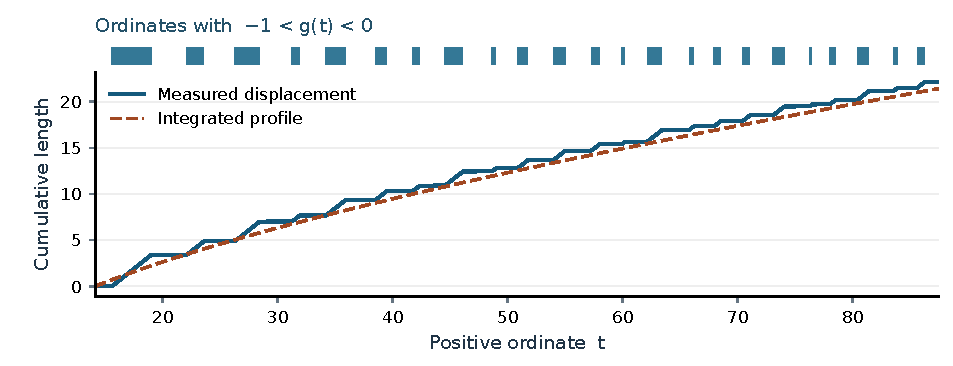
\includegraphics[width=.95\linewidth]{zeta_transport.pdf}
\end{center}
The blue segments mark the 23 transported subintervals. Each segment contributes its length to the cumulative curve below it. For instance the first gap runs from $14.13472514$ to $21.02203964$; the crossings are $15.58570859$ and $18.99408372$. The program uses Hardy's $Z$-function to locate them and checks the logarithmic derivative independently at three interior points. These are floating-point illustrations at low height. The separate rational-arithmetic checks verify the kernel identity and the first three matrix coefficients on two noncommuting examples. The analytic error estimates are established by the proofs above.

\section{Scope, prior work and further questions}\label{sec:prior}
The exact source at the pinned ProveIt revision is \repo{Article/sections/zer.tex}, under \emph{Transport of infinitely many zeros and local Cauchy laws}. Its labels are \texttt{zer:thm:shift}, \texttt{zer:thm:transport}, \texttt{zer:thm:transportexp}, and \texttt{zer:thm:localcauchy}. The Dirichlet GRH input is recorded in \repo{Article/sections/src.tex}. The formalization tracker is \repo{Lean/README.md}. The new endpoint and convergence estimates here are proved in prose. The upstream Lean build was not rerun.

Sodin \cite[\S3.4.5, (55)]{sodin} obtains a weak Cauchy limit for the logarithmic derivative of $\xi$ sampled on $[0,T]$. Najnudel and Nikeghbali \cite{nn} obtain related macroscopic limits using a horizontal-moment condition on zeros. The classical value-distribution theory of Herglotz functions \cite{pearson,aw} and its relation to matrix spectral shift \cite{bmn} explain the appearance of the Cauchy density and the determinant phase. The contribution in \eqref{eq:matrix} is the quantitative sharp-interval remainder, uniform after weighting by the actual size of the matrix phase. The targeted literature comparison did not identify the simultaneous estimate \eqref{eq:scalar} or the finite limit \eqref{eq:global} in these sources. A priority claim beyond this comparison would require a wider review.

\paragraph{How much further can the interval shrink?}
There is a limitation to the analytic input used in Lemma~\ref{lem:strip}. The model $g_k(z)=\cot(kz/2)$ maps the upper half-plane into the lower one and
$(g_k+\ii)/(g_k-\ii)=e^{\ii kz}$. Its distance from $-\ii$ at height one is $O(e^{-k})$. In each period $2\pi/k$, the event $0<g_k<1$ fills a contiguous interval of length $\pi/(2k)$. The standard Cauchy probability of this event is $1/4$. Taking that interval itself as the time window gives discrepancy $3\pi/(8k)$. With $d=e^k$, the size is exactly of order $1/\log d$. This is an obstruction for arguments based only on the Cayley-transform bound; the optimal arithmetic scale for Dirichlet functions remains open.

\newpage
\paragraph{Two further questions.}
Can one compute $C(t_0)$ to certified accuracy for a concrete pair of couplings, with explicit numerical constants in the tail? Can the same endpoint estimate be obtained for mean-spacing-scale windows outside a controlled exceptional set of heights? The latter problem concerns the fine local zero distribution beyond the information used in this paper.

\begin{thebibliography}{9}\small
\bibitem{repo} V. Reshetnikov, \emph{ProveIt}, Generalized Riemann Hypothesis project, revision \texttt{f6b5955e13bc}, retrieved November 27, 2026. \repo{README.md}; \repo{Article/README.md}.
\bibitem{lean} L. Sernau and collaborators, \emph{GRH for Dirichlet $L$-functions, in Lean 4}, based on the Alp\"oge--Claude development, revision \texttt{72fead102f66}. \href{https://github.com/lsernau/grh-lean/tree/72fead102f663d5c7a407964a13dc0cf9d977207}{Pinned source}.
\bibitem{sodin} S. Sodin, \emph{On the critical points of random matrix characteristic polynomials and of the Riemann $\xi$-function}, Q. J. Math. 69 (2018), 183--210. \href{https://arxiv.org/abs/1611.10037}{arXiv:1611.10037}.
\bibitem{nn} J. Najnudel and A. Nikeghbali, \emph{Cauchy laws for zeta logarithmic derivatives and stationary Stieltjes transforms} (2026). \href{https://arxiv.org/abs/2609.15862}{arXiv:2609.15862}.
\bibitem{ccm} E. Carneiro, V. Chandee and M. B. Milinovich, \emph{A note on the zeros of zeta and $L$-functions}, Math. Z. 281 (2015), 315--332. \href{https://arxiv.org/abs/1503.00955}{arXiv:1503.00955}.
\bibitem{pearson} D. B. Pearson, \emph{Value distribution and spectral theory}, Proc. London Math. Soc. (3) 68 (1994), 127--144. \href{https://doi.org/10.1112/plms/s3-68.1.127}{doi:10.1112/plms/s3-68.1.127}.
\bibitem{aw} M. Aizenman and S. Warzel, \emph{On the ubiquity of the Cauchy distribution in spectral problems}, Probab. Theory Related Fields 163 (2015), 61--87. \href{https://arxiv.org/abs/1312.7769}{arXiv:1312.7769}.
\bibitem{bmn} J. Behrndt, M. M. Malamud and H. Neidhardt, \emph{Scattering matrices and Weyl functions}, Proc. London Math. Soc. (3) 97 (2008), 568--598. \href{https://arxiv.org/abs/math-ph/0604013}{arXiv:math-ph/0604013}.
\end{thebibliography}
\end{document}
